\documentclass[10pt,a4paper]{article}
\usepackage[utf8]{inputenc}
\usepackage[english]{babel}
\usepackage{amsmath}
\usepackage{amsfonts}
\usepackage{amssymb}
\usepackage{graphicx}
\usepackage{physics}
\usepackage{stmaryrd}
\usepackage[left=2cm,right=2cm,top=2cm,bottom=2cm]{geometry}
\author{Marco Biroli}
\title{Midterm homework problems}

\begin{document}
\maketitle

\section{Divergence and Laplacian}

\begin{enumerate}

\item We have the definition of Christoffel symbols:
\[
\Gamma_{ij}^k = \pdv{\vb{e}_i}{x^j} \cdot \vb{e}^k
\]
Then we have that:
\[
\div \vb{V} = \partial_i ( V^j \vb{e_j})^i = \pdv{V^i}{x^i} + \Gamma^i_{i j} V^j = V^i_{, i} + \frac{1}{2} g^{im} ( g_{mi, j} + g_{mj, i} - g_{i j, m} ) V^j = {V^i}_{,i} + \frac{1}{2} g^{\mu \nu} g_{\mu \nu, \gamma} V^\gamma
\]

\item Since the determinant is not an invariant scalar the cofactor matrix does not transform as a tensor.

\item We have that:
\[
g = \sum_\nu g_{\mu \nu} c^{\mu \nu} \mbox{~hence~} \pdv{g}{g_{\mu \nu}} = \pdv{}{g_{\mu \nu}} \sum_{\nu'} g_{\mu \nu'} c^{\mu \nu'} = c^{\mu \nu}
\]

\item Following the hint we have that:
\[
\partial_\gamma g = \pdv{g}{g_{\mu \nu}} \partial_\gamma g_{\mu \nu}
\]
Now using the previous questions we can replace this by:
\[
g g^{\mu \nu} g_{\mu \nu, \gamma}
\]
Then up to refactorizing we obtain:
\[
\frac{\partial_\gamma g}{g} = g^{\mu \nu} g_{\mu \nu, \gamma}
\]
Which using the definition of the logarithm gives:
\[
\partial_\gamma \log |g| = g^{\mu \nu} g_{\mu \nu, \gamma}
\]

\item We start from the end and we differentiate to obtain:
\[
\frac{1}{\sqrt{|g|}} \partial_\gamma (\sqrt{|g|} V^\gamma) = {V^\gamma}_{, \gamma} + \frac{1}{\sqrt{|g|}} V^\gamma \frac{1}{2 \sqrt{|g|}} \partial_\gamma |g| = {V^\mu}_{, \mu} + \frac{1}{2} V^\gamma \frac{\partial_\gamma |g|}{|g|} = {V^\mu}_{, \mu} + \frac{1}{2} V^\gamma \log|g|
\]
Now using question 4 we re-obtain the formula of question 1 and this concludes the proof.

\item Using the above formula by replacing: $V_\gamma = f_{, \gamma}$ (hence $V^\gamma = g^{\gamma \mu} f_{,\mu}$) we obtain:
\[
\laplacian f = \frac{1}{\sqrt{|g|}} \partial_\gamma( \sqrt{|g|} f^{,\gamma} ) = \frac{1}{\sqrt{|g|}} \partial_\gamma( \sqrt{|g|} g^{\gamma \mu}f_{,\mu} )
\] 

\item In spherical coordinates we have that:
\[
[g_{\mu \nu}] = \begin{pmatrix}
1 & 0 & 0\\
0 & r^2 & 0 \\
0 & 0 & r^2 \sin^2 \theta 
\end{pmatrix}
\]
Then in order to apply the previous formula we need to compute $g$ and $[g^{\mu \nu}]$. We have quite simply:
\[
g = r^4 \sin^2 \theta \mbox{~~and~~} g^{\mu \mu} = \frac{1}{g_{\mu \mu}} \mbox{~~and~~} g^{\mu \nu} = 0 \mbox{~~otherwise.}
\]
Plugging this in the previous formula we obtain:
\[
\laplacian f = \frac{1}{r^2 \sin \theta} \partial_\gamma(r^2 \sin\theta g^{\gamma \mu} f_{, \mu}) = \frac{1}{r^2 \sin \theta} \left( \partial_r (r^2 \sin \theta f_{,r}) + \partial_\theta (\sin \theta f_{, \theta}) + \partial_\varphi (\frac{1}{\sin \theta} f_{,\varphi}) \right)
\]
Now simplifying the derivatives gives:
\begin{align*}
\laplacian f &= \frac{1}{r^2 \sin \theta} \left( \sin \theta \partial_r (r^2 f_{,r}) + \partial_{\theta} (\sin \theta f_{, \theta}) + \frac{1}{\sin \theta} \partial_\varphi f_{,\varphi}  \right) \\
&= \frac{1}{r^2} \partial_r (r^2 f_{,r}) + \frac{1}{r^2 \sin \theta} \partial_\theta (\sin \theta f_{, \theta}) + \frac{1}{r^2 \sin^2 \theta}\partial_\varphi f_{,\varphi}
\end{align*}

\item Repeating an identical argument but using:
\[
[g_{\mu \nu}] = \begin{pmatrix}
1 & 0 & 0\\
0 & 1 & 0\\
0 & 0 & r^2
\end{pmatrix}
\]
Gives us immediately that:
\[
\laplacian f = \frac{1}{r} \partial_\gamma (r g^{\gamma \mu}f_{, \mu}) = r^{-1} ( \partial_z (r f_{,z} + \partial_{r} (r f_{,r}) + \partial_\phi (r^{-1} f_{,\phi})  ) = f_{,zz} + r^{-1} f_{,r} + f_{,rr} + r^{-2} f_{,\phi\phi}
\]
\end{enumerate}

\section{Rotating coordinate frame.}

\begin{enumerate}

\item We have that:
\[
t = t \mbox{~~and~~} z = z' \mbox{~~and~~} r = r' \mbox{~~and~~} \phi = \phi' - \Omega t
\]
Hence we immediately get that:
\[
\dd t = \dd t \mbox{~~and~~} \dd z = \dd z' \mbox{~~and~~} \dd r = \dd r' \mbox{~~and~~} \dd \phi = \dd \phi' - t \dd \Omega  - \Omega \dd t = \dd \phi' - \Omega \dd t
\]
Where in the last equality we add the assumption that we place ourselves in a rotating frame at constant angular velocity. Now plugging this in the expression for a line element we obtain:
\begin{align*}
\dd s^2 &= -c^2 \dd t^2 + (\dd z')^2 + (\dd r')^2 + (r')^2 (\dd \phi')^2 = - c^2 \dd t^2 + \dd z^2 + \dd r^2 + r^2 (\dd \phi + \Omega \dd t)^2\\
&= - c^2 \dd t^2 + \dd z^2 + \dd r^2 + r^2 \dd \phi^2 + r^2 \Omega^2 \dd t^2 + 2 r^2 \Omega \dd \phi \dd t\\
&= (r^2 \Omega^2 - c^2) \dd t^2 + \dd z^2 + \dd r^2 + r^2 \dd \phi^2 + 2r^2 \Omega \dd t \dd \phi
\end{align*}
Hence we also get:
\[
[g_{\mu \nu}] = \begin{pmatrix}
(r^2 \Omega^2 - c^2) & 0 & 0 & r^2 \Omega\\
0 & 1 & 0 & 0\\
0 & 0 & 1 & 0\\
r^2 \Omega & 0 & 0 & r^2
\end{pmatrix}
\]

\item The inverse can be immediately obtained through it's cofactor formulation and gives:
\[
[g^{\mu\nu}] = \left(
\begin{array}{cccc}
 -\frac{1}{c^2} & 0 & 0 & \frac{\Omega }{c^2} \\
 0 & 1 & 0 & 0 \\
 0 & 0 & 1 & 0 \\
 \frac{\Omega }{c^2} & 0 & 0 & \frac{c^2 - r^2 \Omega ^2}{c^2 r^2} \\
\end{array}
\right) \mbox{~~and~~} g = -c^2 r^2 
\]

\item The line element is given by:
\[
\dd s^2 = - c^2 \dd t^2 + \dd x^2 + \dd y^2 + \dd z^2 
\]
Now as seen in exercise 1 we have that:
\[
\dd s^2 = - c^2 \dd t^2 + \dd r^2 + r^2 \dd \theta^2 + \dd z^2 
\]
Now we are making the change $\theta' = \theta + \Omega t$ hence we obtain:
\[
\dd s^2 = - c^2 \dd t^2 + \dd r^2 + r^2 \dd \theta^2 + r^2 \Omega^2 \dd t^2 + r^2 \Omega \dd \theta \dd t + \dd z^2 
\]
Now replacing back with:
\[
\dd r = \frac{2 \dd x + 2 \dd y}{2\sqrt{x^2 + y^2}} \mbox{~~and~~} \dd \theta = \frac{x\dd y - y \dd x}{x^2 + y^2}
\]
We obtain:
\[
\dd s^2 = -(c^2 - (x^2 + y^2)\Omega^2)\dd t^2 +  \Omega(y \dd x \dd t - x \dd y \dd t) + \dd x^2 + \dd y^2 + \dd z^2
\]

\item We have that:
\[
\begin{pmatrix}
-1 + h_{00} & h_{01} & h_{02} & h_{03}\\
h_{10} & 1 + h_{11} & h_{12} & h_{13}\\
h_{2 0} & h_{21} & 1 + h_{22} & h_{23}\\
h_{30} & h_{31} & h_{32} & 1 + h_{33}
\end{pmatrix}
= 
\begin{pmatrix}
-(1 - (x^2 + y^2) \Omega^2) & \Omega y & -\Omega x & 0\\
\Omega y & 1 & 0 & 0\\
-\Omega x & 0 & 1 & 0\\
0 & 0 & 0 & 1
\end{pmatrix}
\]
Hence we get:
\[
[h_{\mu \nu}] = \begin{pmatrix}
(x^2 + y^2) \Omega^2 & \Omega y/2 & - \Omega x/2 & 0\\
\Omega y/2 & 0 & 0 & 0\\
-\Omega x/2 & 0 & 0 & 0\\
0 & 0 & 0 & 0
\end{pmatrix}
\]
Then the Christoffel's symbols are given by:
\[
[\Gamma^x_{\mu \nu}] = \begin{pmatrix}
- \Omega^2 x & 0 & \Omega/2 & 0\\
0 & 0 & 0 & 0\\
\Omega/2 & 0 & 0 & 0\\
0 & 0 & 0 & 0
\end{pmatrix} \mbox{~~and~~} [\Gamma^y_{\mu \nu}] = \begin{pmatrix}
- \Omega^2 y & - \Omega/2 & 0 & 0\\
- \Omega/2 & 0 & 0 & 0\\
0& 0 & 0 & 0\\
0 & 0 & 0 & 0
\end{pmatrix}
\]

\item Then the equations of motions are given by the equation for a geodesic:
\[
\dv[2]{x^\mu}{\tau} + \Gamma^\mu_{\nu \gamma} \dv{x^\nu}{\tau} \dv{x^\gamma}{\tau} = 0
\]
Which when we plug in the values of the Christoffel's symbols we get:
\[
\begin{cases}
\ddot{x} = \Omega (\Omega x -  \dot{y})\\
\ddot{y} = \Omega(\Omega y +  \dot{x})
\end{cases}
\]

\end{enumerate}

\section{Frame dragging by a moving rod.}

\begin{enumerate}

\item We have the equation:
\[
\laplacian \Phi = 4\pi (G_N/c^2) \rho \Theta(R - r)
\]
From symmetry arguments we know already that $\Phi$ will only be a function of $r$. Hence we have that by plugging the expression of the laplacian found in part 1 we obtain:
\[
\Phi_{,zz} + \Phi_{,rr} + \Phi_{,r}/r + \Phi_{,\phi\phi}/r^2 = \Phi_{,rr} + \Phi_{,r}/r =  4 \pi (G_N/c^2) \rho
\]
This can be re-written as:
\[
\partial_r(r \Phi_{,r}) = 4 \pi (G_N /c^2)\rho r \Rightarrow r \Phi_{,r} = 4\pi (G_N/c^2) \rho r^{2}/2 + c
\]
Which gives immediately through integration a solution of the form:
\[
\Phi(r) = \pi (G_N/c^2) \rho r^2  + c \log(r) + c'
\]
Now the condition $\Phi_{,r}(0) = 0$ ensures that $c = 0$ and the condition $\Phi(R) = 0$ ensures that $c' = - \pi (G_N/c^2) \rho R^2$ hence the final solution is given by:
\[
\Phi(r) = \pi(G_N/c^2)\rho(r^2 - R^2)
\]

\item We have that:
\[
\overline{h_{\mu \nu}} = -4 \Phi \delta^0_\mu \delta^0_\nu
\]
Hence we get that:
\[
h_{\mu \nu} - \frac{1}{2} \eta_{\mu \nu} h = - 4 \Phi \delta^0_\mu \delta^0_\nu
\]
Now we have that:
\[
\eta_{\mu\nu}(\overline{h}_{\mu\nu}) = h - \frac{1}{2} Tr(\eta) h = h - 2h = - h
\]
Which when plugged in the previous equation gives immediately that:
\[
-h = 4 \Phi \Leftrightarrow h = -4 \Phi
\]
Hence we obtain that:
\[
h_{\mu \nu}(r) = - 2 \Phi \delta_{\mu \nu}
\]


\item We have that:
\[
\dd s^2 = (1 - 2 \Phi) (\dd r^2 + r^2 \dd \phi^2)
\]
Now we apply the following transformations:
\[
r' = (1 + r \Phi_{,r})(1 - \Phi) r  \mbox{~~and~~} \phi' = (1 - \Phi_{,r}/r)\phi
\]
Now inserting the expression of $\Phi$ that we found above we get that:
\[
r' = r(\frac{1}{2} - \alpha/4)(2 - \alpha \log(r/R)) 
\]
Then inserting the differentials and linearizing to first order gives the desired result.

\item
\begin{enumerate}
\item We have that:

\[
[\Lambda^\mu_{\nu}] = \begin{pmatrix}
\gamma & 0 & 0 & \beta \gamma\\
0 & 1 & 0 & 0\\
0 & 0 & 1 & 0\\
\beta \gamma & 0 & 0 & \gamma
\end{pmatrix}
\]

\item Consider a particle at rest then we have that:
\[
\vb{x} = (ct \quad 0 \quad 0 \quad 0)^T
\]
Applying the tensor above we get:
\[
[\Lambda^\mu_\nu x^\nu] = \begin{pmatrix}
ct \gamma \\
0 \\
0 \\
\beta \gamma c t 
\end{pmatrix}
\]

\item We have that $t_{\alpha \beta}x^\alpha x^\beta$ is a scalar hence it is invariant under a Lorentz transformation. Therefore we can write:
\[
t_{\alpha \beta} x^\alpha x^\beta = t_{\alpha' \beta'} \Lambda^{\alpha'}_\alpha x^{\alpha} \Lambda^{\beta'}_\beta x^{\beta}
\]
Hence we immediately get that:
\[
t_{\alpha' \beta'} = (\Lambda^{-1})^{\alpha'}_{\alpha} (\Lambda^{-1})^{\beta'}_\beta t_{\alpha \beta}
\]
Where the inverse can be easily found since $L(\beta)^{-1} = L(-\beta)$. 

\item Then the perturbation to the metric is expressed as :
\[
[h_{\alpha'\beta'}] = 4 \pi \frac{G_N}{c^2} \rho \log(\frac{r}{R}) \begin{pmatrix}
\frac{c^2 + v^2}{c^2 - v^2} & 0 & 0 & -\frac{2 c v}{c^2 - v^2}\\
0 & 1 & 0 & 0\\
0 & 0 & 1 & 0\\
-\frac{2 c v}{c^2 - v^2} & 0 & 0 & \frac{c^2 + v^2}{c^2 - v^2}
\end{pmatrix}
\]


\end{enumerate}


\item  A first order Taylor expansion in $\beta$ quickly yields:
\[
[h_{\alpha' \beta'}] = 4 \pi \frac{G_N}{c^2} \rho \log(\frac{r}{R}) \begin{pmatrix}
1 & 0 & 0 & - 2 \beta\\
0 & 1 & 0 & 0\\
0 & 0 & 1 & 0\\
-2 \beta & 0 & 0 & 1
\end{pmatrix}
\]

\item \begin{enumerate}

\item We use the geodesic equation:
\[
-\dv[2]{z}{\tau} = \Gamma^z_{\mu \nu} \dv{x^\mu}{\tau} \dv{x^\nu}{\tau}
\]
Then:
\[
\Gamma^\nu_{\mu \lambda} = \frac{1}{2}\eta^{\nu \gamma}(\partial_\mu h_{\gamma \lambda} + \partial_{\lambda} h_{\gamma \mu} - \partial_\gamma h_{\lambda \mu})
\]
We start by computing the Christoffel symbols:
\begin{align*}
\Gamma^z_{00} &= \frac{1}{2} \eta^{z \gamma}( \partial_0 h_{\gamma 0} + \partial_0 h_{\gamma 0} - \partial_\gamma h_{00}) = \partial_0 h_{z 0} - \frac{1}{2} \partial_z h_{0 0} = \partial_0 4 \Phi(r) v /c + \partial_z \Phi(r) = 0\\
\Gamma^z_{0 1} &= \frac{1}{2} \eta^{z \gamma} (\partial_0 h_{\gamma 1} + \partial_1 h_{\gamma 0} - \partial_\gamma h_{10}) = \frac{1}{2}(\partial_0 h_{z 1} + \partial_1 h_{z 0} - \partial_z h_{10}) = \frac{1}{2}(0 + \partial_x 4 \Phi(r) v /c + 0) = 2 v /c\,  \partial_x \Phi(r)\\
\Gamma^z_{02} &= \frac{1}{2}(\partial_0 h_{z2} + \partial_2 h_{z0} - \partial_z h_{20}) = 2v/c\, \partial_y \Phi(r)\\
\Gamma^z_{0 3} &= \frac{1}{2}(\partial_0 h_{z3} + \partial_3 h_{z3} - \partial_z h_{30} ) = \frac{1}{2}(-2\partial_z \Phi(r) - 4v/c \partial_z \Phi(r) ) = -(1 - 2v/c) \partial_z \Phi(r) = 0\\
\Gamma^z_{11} &= \frac{1}{2} (\partial_1 h_{z 1} + \partial_1 h_{z 1} - \partial_z h_{11}) =  \partial_z \Phi(r) = 0 \\
\Gamma^z_{12} &= \frac{1}{2}(\partial_1 h_{z 2} + \partial_2 h_{z 1} - \partial_z h_{21}) = 0\\
\Gamma^z_{13} &= \frac{1}{2}( \partial_1 h_{z3} + \partial_3 h_{z1} - \partial_z h_{31} ) = - \partial_x \Phi(r)\\
\Gamma^{z}_{22} &= \frac{1}{2}(\partial_2 h_{z2} + \partial_2 h_{z2} - \partial_z h_{22}) = \partial_z \Phi(r) = 0\\
\Gamma^{z}_{23} &= \frac{1}{2}(\partial_2 h_{z 3} + \partial_3 h_{z2} - \partial_z h_{32}) = - \partial_y \Phi(r)\\
\Gamma^z_{33} &= \frac{1}{2} (\partial_{3} h_{z3} + \partial_3 h_{z3} - \partial_z h_{33}) = 0
\end{align*}
Hence the geodesic equation becomes:
\[
-\ddot{z} = \Gamma^z_{01} \dv{t}{\tau} \dv{x}{\tau} + \Gamma^z_{02} \dv{t}{\tau} \dv{y}{\tau} + \Gamma^z_{13} \dv{x}{\tau}\dv{z}{\tau} + \Gamma^z_{23} \dv{y}{\tau}\dv{z}{\tau}
\]
Plugging in the values we get:
\[
-\ddot{z} = 2v/c( \partial_x \Phi(r) \gamma \dot{x} + \partial_y \Phi(r) \dot{t} \dot{y}) - \dot{z}( \dot{x} \partial_x \Phi(r)  + \dot{y}\partial_y \Phi(r)  )  = (\dot{\vb{x}} \cdot \grad \Phi) (\frac{2v}{c} \gamma - \dot{z}) = \dot{x} \partial_x \Phi (\frac{2v}{c} \dot{t} - \dot{z})
\]
Where in the last equality we used the fact that $\dot{y} = y = 0$ and $\partial_z\Phi = 0$. Now a similar derivation for $\Gamma^t_{\mu \nu}$ and $\Gamma^x_{\mu \nu}$ yields:
\[
-\ddot{t} = \frac{2 v}{c} \dot{z} \dot{x} \partial_x \Phi \mbox{~~and~~}  -\ddot{x} = \partial_x \Phi (\dot{t}^2 - \dot{x}^2 + \dot{z}^2)
\]
Hence the final system of equation gives:
\[
\begin{cases}
-\ddot{z} = \dot{x} \partial_x \Phi \left( \frac{2v}{c} \dot{t} - \dot{z} \right)\\
-\ddot{t} = \frac{2v}{c} \dot{z}\dot{x} \partial_x \Phi\\
-\ddot{x} = \partial_x\Phi (\dot{t}^2 - \dot{x}^2 + \dot{z}^2)
\end{cases}
\]
Now we can also replace $\partial_x \Phi$ by its value: $\frac{2 G_N \pi \rho }{c^2 x}$ (outside of the cylinder) which gives:
\[
\begin{cases}
-\ddot{z} = \dot{x} \frac{2 G_N \pi \rho}{c^2 x} \left( \frac{2v}{c} \dot{t} - \dot{z} \right)\\
-\ddot{t} = \frac{2v}{c} \dot{z}\dot{x} \frac{2 G_N \pi \rho}{c^2 x}\\
-\ddot{x} = \frac{2 G_N \pi \rho}{c^2 x} (\dot{t}^2 - \dot{x}^2 + \dot{z}^2)
\end{cases}
\]
Which when solved numerically gives the figures plotted below.
\begin{figure}[h!]
\centering
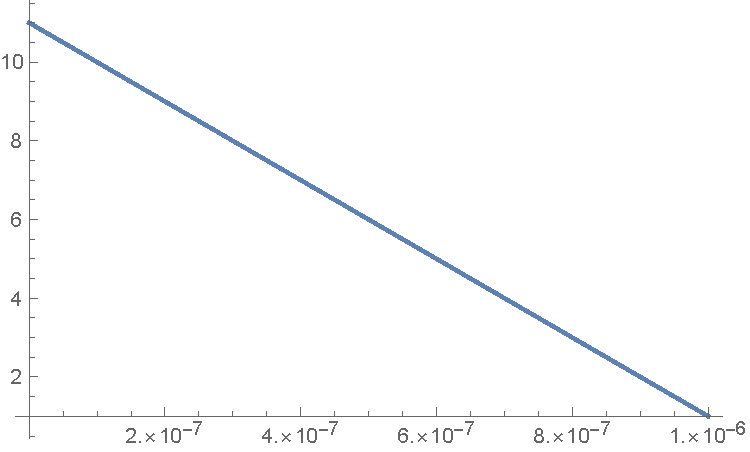
\includegraphics[width = 0.4\textwidth]{fig2}
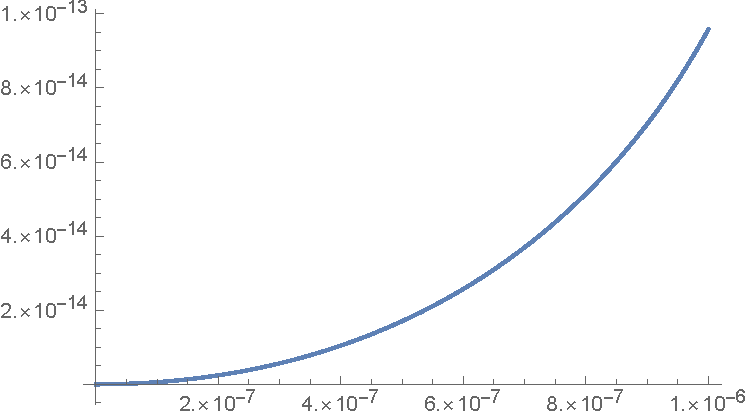
\includegraphics[width = 0.4\textwidth]{fig1}
\caption{Plot of $x(\tau)$ on the left and $z(\tau)$ on the right.}
\end{figure}

\end{enumerate}


\end{enumerate}

\section{Frame-dragging inside a rotating cylinder.}

\begin{enumerate}

\item Consider $V$ to be a cylinder of height $H$ and radius $r$ around the origin. Then from Gauss's law we have that:
\[
2 \pi r H \grad \Phi(r) = \oint_{\partial V} \grad \Phi \dd \vb{S} = \int_V \div \grad \Phi \dd V = \int_V \frac{4 \pi G_N}{c^2} \rho(\vb{x}) \dd V = \frac{4\pi G_N}{c^2} \dd \mu H  
\]
Hence up to re-writing we obtain:
\[
\grad \Phi(r) = \frac{2 G_N}{r c^2} \dd \mu \vu{r}
\]

\item Notice that we can re-write this as:
\[
\div (\grad \Phi_{\mu\nu}) = 4 \pi \kappa T_{\mu \nu} \Leftrightarrow \vb{L} \cdot \vb{u} = f
\]
Now the Green function for a needle pointing along the $z$-axis at position $\vb{x'} = (x, y)$ is given by:
\[
\div \vb{G(\vb{x}, \vb{x'})} = \delta(\vb{x} - \vb{x'}) \Rightarrow \vb{G}(\vb{x}, \vb{x'}) = \frac{1}{2\pi} \frac{\vb{x} - \vb{x'}}{|\vb{x} - \vb{x'}|^2}
\]
Hence we have that the solution $\vb{u} = \grad\Phi_{\mu\nu}$ to the equation $\vb{L} \cdot \vb{u} = f$ is given by:
\[
\grad \Phi_{\mu\nu} = \vb{u} = \int G(\vb{x}, \vb{x'}) f(\vb{x'}) \dd^2 \vb{x'} = \int \frac{\vb{x} - \vb{x'}}{|\vb{x} - \vb{x'}|^2} 2 \kappa T_{\mu\nu}(\vb{x'}) \dd^2 \vb{x'} 
\]

\item We have that (in cylindrical coordinates):
\[
[T_{\mu \nu}] = \rho c^2 \begin{bmatrix}
1 & \vb{v}/c\\
\vb{v}/c & 1
\end{bmatrix} = \rho c^2 \begin{bmatrix}
1 & 0 & \Omega R /c & 0\\
0 & 0 & 0 & 0\\
\Omega R/c & 0 & 0 & 0\\
0 & 0 & 0 & 0
\end{bmatrix}
\]
Then to get it in cartesian coordinates we simply have to compute:
\begin{align*}
[T_{\mu \nu}] &= \rho(\vb{r}) c^2 \begin{bmatrix}
1 & 0 & 0 & 0\\
0 & \cos \theta & -\sin\theta & 0\\
0 & \sin \theta & \cos \theta & 0 \\
0 & 0 & 0 & 1
\end{bmatrix} \begin{bmatrix}
1 & 0 & \Omega R /c & 0\\
0 & 0 & 0 & 0\\
\Omega R/c & 0 & 0 & 0\\
0 & 0 & 0 & 0
\end{bmatrix}\begin{bmatrix}
1 & 0 & 0 & 0\\
0 & \cos \theta & \sin\theta & 0\\
0 & -\sin \theta & \cos \theta & 0 \\
0 & 0 & 0 & 1
\end{bmatrix}\\
&= \rho(\vb{r}) c \Omega R \begin{bmatrix}
\frac{c}{R \Omega} & -\sin\theta & \cos\theta & 0\\
-\sin\theta & 0 & 0 & 0\\
\cos\theta & 0 & 0 & 0\\
0 & 0 &0 &0 
\end{bmatrix}
\end{align*}
Now since we are dealing with a thin-walled cylinder we have that:
\[
\rho(\vb{r}) = \frac{\rho}{2\pi R} \delta(r - R) 
\]
Hence replacing up top we obtain:
\[
[T_{\mu\nu}] = \frac{c \rho \Omega \delta(r - R)}{2\pi} \begin{bmatrix}
\frac{c}{R \Omega} & -\sin\theta & \cos\theta & 0\\
-\sin\theta & 0 & 0 & 0\\
\cos\theta & 0 & 0 & 0\\
0 & 0 &0 &0 
\end{bmatrix}
\]
Then using the equation of the previous question we obtain:
\begin{align*}
\grad \Phi_{0 1}(\vb{0}) &= 2 \kappa \int \dd^2 \vb{x'} T_{0 1}(\vb{x'}) \frac{\vb{0} - \vb{x'}}{|\vb{0} - \vb{x'}|^2} = -2 \kappa \int \dd^2 \vb{x'} \frac{c \rho \Omega \delta(x' - R)}{2 \pi} \sin \theta \frac{\vb{x} - \vb{x'}}{|\vb{x} - \vb{x'}|^2}\\
&= \frac{2 \kappa c \rho \Omega}{2\pi R} \int_0^{2\pi} R \sin \theta \dd \theta = \frac{\kappa c \rho \Omega}{\pi} \int_0^{2\pi} \binom{\sin \theta \cos \theta}{\sin^2\theta} \dd \theta = \kappa c \rho \Omega \vu{y}
\end{align*}
Similarly we have that:
\begin{align*}
\grad \Phi_{02}(\vb{0}) = 2 \kappa \int \dd^2 \vb{x'} \frac{c \rho \Omega \delta(x' - R)}{2 \pi} \cos \theta \frac{\vu{r}}{|\vb{x'}|^2}= -\frac{\kappa c \rho \Omega}{\pi} \int_{0}^{2\pi} \binom{\cos^2\theta}{\sin\theta\cos\theta} \dd \theta = - \kappa c \rho \Omega \vu{x}
\end{align*}

\item \begin{enumerate}

\item We have that:
\[
\Phi_{\mu\nu} = - \overline{h_{\mu\nu}}/4 
\]
From the previous question we also know that:
\[
[\Phi_{\mu\nu}(\vb{x})] = \kappa c \rho \Omega \begin{bmatrix}
0 & y + \ell & - x + \ell' & 0\\
y + \ell & 0 & 0 & 0\\
-x + \ell' & 0 & 0 & 0\\
0 & 0 & 0 & 0
\end{bmatrix}
\]
Then for $[\Phi(\vb{0})] = \vb{0}$ we simply need to take $\ell = \ell' = 0$. Then we have that:
\[
[\overline{h_{\mu\nu}}(\vb{x})] = 4\kappa c \rho \Omega \begin{bmatrix}
0 & - y & x & 0\\
-y & 0 & 0 & 0\\
x & 0 & 0& 0\\
0& 0 & 0& 0
\end{bmatrix}
\]
Then since $\overline{h}_{\mu\nu}$ is traceless we also have that $[h_{\mu\nu}] = [\overline{h}_{\mu\nu}]$. 

\item We have the following expression for the Christoffell symbols, derived similarly as in the 3rd part:
\begin{align*}
\Gamma^t_{\mu \nu} = 0 \mbox{~~and~~} \Gamma^x_{0 2} = -4 c \kappa \rho \Omega  \mbox{~~and~~} \Gamma^y_{0 1} = 4 c \kappa \rho \Omega \mbox{~~and~~} \Gamma^z_{\mu \nu} = 0
\end{align*}
Where the unmentioned values of $\Gamma^x$ and $\Gamma^y$ are zero (apart from the symmetric values). This gives the following equations:
\[
\begin{cases}
\ddot{x} - 8 c \kappa \rho \Omega \dot{y} = 0\\
\ddot{y} + 8 c \kappa \rho \Omega \dot{x} = 0
\end{cases}
\]
Now for simplicity we call $\alpha = 8 c \kappa \rho \Omega$ then we have that the solutions are given by:
\[
x(\tau) = \frac{v_y - v_y  \cos(t\alpha) + v_x \sin(t\alpha)}{\alpha} \mbox{~~and~~} y(t) = \frac{v_x \cos(t\alpha) - v_x + v_y \sin(t \alpha)}{\alpha}
\]
Where $(v_x, v_y)$ are the initial velocities of the particle. We can see from the above equations that these are the parametric equations for a circle of center $c = (\frac{v_y}{\alpha}, -\frac{v_x}{\alpha})$ and of radius:
\[
r = \frac{\sqrt{v_x^2 + v_y^2} \sin(4 c t \kappa \rho \Omega)}{8 c \kappa \rho \Omega} = \frac{\sin(t \alpha/2)}{\alpha} \sqrt{v_x^2 + v_y^2}
\]
We hence will obtain a periodic opening and closing orbit around $c$. 

\item Consider a second still object at an arbitrary position in space. Then if we change to a rotating frame the cylinder might have stopped spinning however the other object will have started spinning. 

\end{enumerate}

\end{enumerate}

\end{document}